% 1) Overarching Questions  What I want to know?
% 2) Measurements (MEADcast specific) How can I measure that
% 3) Scenarios
%    3.1) Potential Application Domains
%    3.2) Application Characteristics
% 4) Experiments
% 5) Parameters
\chapter{Experiment Design} % (fold)
\label{chap:Design}
This chapter addresses the design of a series of experiments to evaluate
    MEADcast.
To ensure the quality of the experiments \autoref{sec:Measurements} discusses
    research questions driving our design process.
Subsequently, \autoref{sec:Scenarios} elaborates on motivations for employing
    multicast, potential application domains and their characteristics.
This chapter deals with the selection of measurements, design of experiments
    and the design of a testbed based on requirements derived from the
    experiments.

Based on thesis goal we first formulate overarching research questions we
    endeavour to answer with our experiments. 
Therefore, these questions guide our design process of the experiments.
% Feasibility:
% - How robust is the current MEADcast specification?
% - Are there any issues or opportunities for improvement with the current 
%   protocol specification

% Performance:
% - How does MEADcast perfom compared to unicast and IP-Multicast
% - How big is the overhead of the discovery phase?
% - How does the degree of deployed MEADcast routers impact the results?

% Scenarios:
% - Under which conditions is the usage of MEADcast sensible?
% - Which applications and characteristics are well served by MEADcast?


\section{Measurements} % (fold)
\label{sec:Measurements}
% Based on the thesis goal we first formulate overarching research questions we
%     endeavor to answer with our experiments. 
% Therefore, these questions guide our design process for the experiments.
% Following, this section depicts how we answer these questions.
Aligned with the goal of this thesis, we begin by formulating  overarching
    research questions, guiding the design of the experiments.
Additionally, this section outlines our approach to answering these questions.

\begin{enumerate}
    \item[\textit{RQ1}]
        \textit{How robust is the current MEADcast specification?}\par
        While prior research on MEADcast has primarily taken place in simulated
            environments \cite{meadcast1, meadcast2} and small stub networks
            \cite{sdn_ba}, this thesis endeavors to assess MEADcast in a more
            realistic setting.
        To achieve this, we perform a stress test to evaluate the protocol's
            behavior in a less ``clinical'' environment.
        During this test we observe MEADcast's reaction to deliberate routing
            changes, to evaluate its adaptivity and suitability for dynamic
            network environments.
        Further, we simulate network disruptions by inducing router outages, to
            assess MEADcast's resilience and recovery capabilities.
        The stress test also examines MEADcast anomaly handling by injecting
            modified discovery responses.
        Additionally, a firewall is employed to intentionally drop MEADcast
            packets during the data delivery phase, enabling us to evaluate the
            efficacy of the fallback mechanism.
        The results of the stress test shed light on the robustness of the
            current MEADcast specification, especially in diverse network
            conditions.
        This investigation aims to provide valuable insights into the
            real-world applicability and resilience of MEADcast.
    \item[\textit{RQ2}]
        % typical metrics: throughput, latency, jitter, resource utilization,
        %   ... in different scenarios
        % impact of the discovery phase
        \textit{How does MEADcast perform compared to IP-Unicast and
        IP-Multicast?}\par
        In addition to assessing the robustness of a protocol, its performance,
            especially in comparison to existing alternatives, is a pivotal
            factor influencing its adoption.
        To address this research question, comparative performance measurements
            for MEADcast, IP-Unicast, and IP-Multicast are conducted across a
            series of experiments elaborated in \autoref{sec:Scenarios}.
        These measurements encompass metrics such as throughput, latency,
            jitter, and resource utilization.
        Special attention is given to the impact of MEADcast's discovery phase
            on its performance.
        This encompasses assessing the overhead produced by the discovery
            mechanism.
        Furthermore, we evaluate how the protocol's shift from extensive
            unicast to MEADcast delivery affects the performance metrics.
        The outcomes contribute not only to evaluating MEADcast performance but
            also to drawing conclusions for subsequent research questions.
    \item[\textit{RQ3}]
        \textit{Which applications and characteristics are well served by
        MEADcast?}\par
        % first look at motivations, application domains and characteristics
        % for multicast. Then select scenarios to portray a variety
        Addressing this research question involves designing a series of 
            experiments depicting a diverse range of applications with distinct
            characteristics (see \autoref{sec:Scenarios}).
        The selection of scenarios is guided by an initial exploration of
            motivations for employing multicast communication, and more
            specifically, MEADcast.
        These motivations lay the groundwork for identifying a range of
            potential application domains where MEADcast deployment could prove
            beneficial.
        Subsequently, we formulate application characteristics distinguishing
            these domains.
        Based on the gathered insights, various scenarios are chosen to
            represent different application domains and their unique set of
            characteristics.
        This comprehensive selection ensures a throughout examination of
            MEADcast's suitability across a diverse spectrum of use cases.
        The results aim to delineate MEADcast's application space by
            identifying its strengths and limitations.
    \item[\textit{RQ4}] \label{itm:RQs}
        \textit{In which conditions is the usage of MEADcast sensible?}\par
        % testing parameters based on scenarios
        % Number of EPs
        % Number of MEADcast routers
        % EP distribution
        % Available Bandwidth
        The viability of employing MEADcast is influenced not only by
            application domains and their characteristics but also by
            prevailing circumstances.
        To investigate this aspect, the experiments are executed with various
            parameter configurations.
        For instance, the level of network control and the number of available
            MEADcast routers affect the performance and thus the viability of
            MEADcast.
        This applies equally to testing parameters like available bandwidth,
            number of endpoints, and their distribution.
        % Further testing parameters are the available bandwidth, the number of
        %     receivers, and their distribution.
        The goal is to provide insights into the conditions under which
            deploying MEADcast is advantageous compared to existing
            alternatives.
        The results aim to offer guidance for making informed decisions
            regarding the adoption of MEADcast in specific circumstances.
        % The results aims to provide guidance, under which circumstances
        %     employing MEADcast is favorable in comparison to existing
        %     alternatives.
\end{enumerate}




\section{Scenarios} % (fold)
\label{sec:Scenarios}
% Questions
% Motivation
% Characteristics
% Domains
% Experiments
% Parameters

% Char -> Domain
% To design comparable experiments we have to elaborate characteristics of 
%     applications that may benefit from Multicast-Communication.
% Based on these characteristics, we formulate potential application domains for
%     Multicast-Communication.
% Lastly, a series of experiments is depicted.

To design comparable experiments we have to elaborate on application domains
    that may benefit from Multicast-Communication.
Following, we formulate application characteristics distinguishing these
    domains.
This knowledge enables us to design a series of experiments representing
    a variety of application domains with differing characteristics.
Thereby we aim to answer RQX.

\subsection{Motivations for employing Multicast} % (fold)
\label{sub:MotivationsForMulticast}
To select appropriate measurements and experiments, it is essential to delve
    into the \textit{motivations} for employing multicast communication and,
    specifically, MEADcast as a protocol.

% Motivations to use Multicast:
% Efficient resource usage, to...
%   - Overcome resource limitation (technical or financial cause)
%       Technical: no more upstream available,
%           ip cam can't handle streaming to multiple receivers
%       Financial: don't want to pay more for: IPS upstream, cloud egress, VPN, ...
%                   or just reduce costs
%   - use traffic intense services, despite ones bandwidth limitation
%   - facilitate new services or improve existing ones
%   - Emissions
In a broader context, the decision to utilize multicast often resolves around
    optimizing resource usage.
In the absence of resource constraints, one might question opting for multicast
    rather than ubiquitous unicast communication.
However, several compelling reasons advocate for the adoption of a multicast
    protocol.
A predominant motive is overcoming \textit{resource limitations}, which can
    manifest technically, such as a network connection incapable of providing
    the required bandwidth, or \gls{iot} devices like IP cameras struggling
    to handle numerous unicast connections requesting identical content.

Financial considerations are also a driving reason for employing multicast,
since most internet services operate on a subscription or pay-as-you-go pricing
    model (pay per usage).
\glspl{isp}, mobile phone operators, and VPN providers structure their services
    based on factors like monthly available traffic volume, upstream and
    downstream bandwidth.
Subscribed service levels can thus become the financial cause of resource
    limitations.
Cloud providers, in particular, heavily rely on pay-as-you-go pricing, often
    contending their customers with expensive ``egress costs''.
Deploying multicast emerges as a strategic approach to not only overcome
    technical and financial constraints but also to reduce operational costs.

Another motivation for multicast adoption is to facilitate new services or 
    enhance existing ones.
For example, employing multicast for delivering multimedia content enables
    service providers to offer higher-quality audio or video without the need
    to either increase operational costs or overcome prevailing resource
    limitations.
Moreover, multicast can empower individuals to access bandwidth-intensive
    services despite their limited bandwidth.
For instance, \gls{p2p} conferencing services could leverage multicast to
    bridge the asymmetric access link common in most households (high
    downstream and low upstream bandwidth) \cite{xcast_rfc}.
Additionally, network operators may strategically deploy multicast within their
    domain to decrease overall network load, concurrently reducing operational
    costs and mitigating emissions caused by \gls{ct} (see
    \autoref{sec:Motivation}).

% Motivations for choosing MEADcast as Multicast protocol:
% - IP Multicast often no real option
% - Limited network control (fallback)
% - No deployment of specialized client software
% - Protect receiver privacy
% - Access control to multicasted content
As constituted in \autoref{sec:Challenges of Multicast} and
    \autoref{sub:IP Multicast}, in many scenarios, the usage of IP-Multicast
    is not a viable option.
This creates a potential application space for MEADcast, particularly in
    circumstances with limited network control and an uncertain degree of
    IP-Multicast support.
Another potential domain for MEADcast is in facilitating access control-based
    multicast communication, addressing the absence of a receiver authorization
    mechanism in IP-Multicast \cite{diot2000deployment}.
In comparison to alternatives like Xcast or \gls{alm}, MEADcast might be
    favored in situations where the disclosure of receiver information, such as
    IP addresses, among other group members, is deemed unacceptable.
% subsection Motivations (end)


\subsection{Application Domains} % (fold)
\label{sub:Application Domains}
As highlighted in the preceding section, numerous motivations support the
    adoption of multicast communication.
Additionally, various types of applications have the potential to benefit
    from multicast communication.
% Furthermore, there are various kinds of applications, which potentially benefit
%     from Multicast.
% However, as outlined in \autoref{tab:mccomm} multicast is specifically tailored
%     for a particular form of communication -- \textit{simultaneous}
%     transmission of \textit{identical} data to multiple recipients.
However, it is essential to acknowledge that multicast is tailored for a
    specific form of communication -- \textit{simultaneous} transmission of 
    \textit{identical} data to multiple recipients, as delineated in
    \autoref{tab:mccomm}.
This inherent characteristic finds an ideal match in TV broadcasts,
    establishing them as a prime candidate for multicast communication.
Conversely, Video on Demand services such as YouTube present a less favorable
    scenario for multicast adoption, as users request videos at different
    points in time.
The advantages of multicast become particularly evident in bandwidth-intense
    applications, where its potential to significantly reduce the total
    communication volume is most pronounced.
Real-time multimedia services, therefore, emerge as a particularly well-suited
    domain for the application of multicast.
In the following, we introduce the formulated application domains, illustrating
    them with specific examples as detailed in \autoref{tab:mcappdom}.
The characteristics distinguishing these domains are discussed in the
    following section.

\begin{table}
    \centering
    \begin{tabular}{ccc}
    \toprule
        & \multicolumn{2}{c}{\textbf{Temporal}} \\
        \cmidrule{2-3}
        \textbf{Content} & Synchronous & Asynchronous \\
    \midrule
        Identical & TV broadcast & Video on demand \\
                  & (yes)        & (no) \\
        \addlinespace
        Different & -            & Web browsing \\
                  & (no)         & (no) \\
        % Identical & yes & no \\
        % Different & no & no \\
    \bottomrule
    \end{tabular}
    \caption{Suitability of communication patterns for Multicast}
    \label{tab:mccomm}
\end{table}

The first application domain is \textit{Multimedia Streaming}, encompassing 
    various applications transmitting multimedia content to an arbitrary number
    of destinations, such as IPTV \cite{meadcast2, ratnasamy2006revisiting},
    Internet Radio \cite{meadcast1}, podcasts, and live streaming (e.g.
    Twitch).
\textit{Conferencing and Collaboration} is the second domain, comprising Audio
    and Video Conferences \cite{overlay_mc_routing, meadcast2,
    mc_routing_multimedia}, \gls{voip} \cite{gxcast, xcast_rfc}, as well as
    real-time collaboration applications \cite{diot2000deployment, xcast_rfc}
    like online Mind Maps and Whiteboards.
The next domain \textit{File Transfer}, covers numerous applications 
    distributing files to multiple recipients, including Software Distribution
    and Updates, Patch Management \cite{meadcast1, ratnasamy2006revisiting}, 
    Logging \cite{diot2000deployment} as well as file sharing and
    synchronization \cite{overlay_mc_routing}.
\textit{Information delivery} comprises applications pushing information to 
    multiple destinations.
One example is a news application, which notifies it's users about new
    information of topics or channels they have subscribed
    \cite{diot2000deployment}.
Other applications include widely utilized smartphone notifications, RSS feeds
    \cite{ratnasamy2006revisiting}, Logging (e.g. SNMP), and Stock quotes
    \cite{cisco_ipmc}.
The last domain is \textit{Distributed Simulation}, with exemplary applications
    such physics simulations \cite{diot2000deployment}, virtual reality, and
    online gaming \cite{ratnasamy2006revisiting}.

% \textit{Multimedia streaming} presents the first application domain.
% This domain comprises various applications transmitting multimedia content to 
%     an arbitrary number of destinations, such as IPTV \cite{meadcast2,
%     ratnasamy2006revisiting}, Internet Radio \cite{meadcast1},
%     podcasts, and live streaming (e.g. Twitch).
% The next application domain is \textit{Conferencing and Collaboration},
%     encompassing Audio- and Video-Conferences \cite{overlay_mc_routing,
%     meadcast2, mc_routing_multimedia}, \gls{voip} \cite{gxcast, xcast_rfc},
%     as well as real-time collaboration tools \cite{diot2000deployment,
%     xcast_rfc} like Mind Maps and Whiteboards.
% Another domain is \textit{File Transfer}.
% This includes all forms of distributing files to multiple recipients.
% Prominent examples are Software-Distribution and -Updates and Patch Management
%     \cite{meadcast1, ratnasamy2006revisiting}, Logging
%     \cite{diot2000deployment} as well as file-sharing and -synchronization
%     \cite{overlay_mc_routing}.
% The next application domain is \textit{Information delivery}.
% This comprises information that gets pushed to multiple destinations.
% For example, in a news application users could subscribe to certain topics or
%     channels they want to receive updates from \cite{diot2000deployment}.
% Further applications are widely used smartphone notifications, RSS feeds
%     \cite{ratnasamy2006revisiting}, Logging (e.g. SNMP), and Stock quotes
%     \cite{cisco_ipmc}.
% The last domain is called \textit{Distributed simulation}.
% Exemplary applications are physics simulations, virtual reality
%     \cite{diot2000deployment}, and online gaming \cite{ratnasamy2006revisiting}.



%\cite{overlay_mc_routing}:
%   - video conference,
%   - video on demand
%   - distributed simulation (incl. online gaming)
%   - p2p file sharing

%\cite{mc_routing_multimedia}
%   - audio and video

%\cite{meadcast1, meadcast2}
%   - Audio and Video Conferencing
%   - IPTV, Internet Radio
%   - Sofware updates
%   - large scale Configuration

%\cite{diot2000deployment}
%    - real time audio and video
%    - Push applications
%    - Conferencing and Collaboration
%    - File tranfser (cache, logging)

%\cite{ratnasamy2006revisiting}
%    - Online Games
%    - IPTV
%    - File sharing
%    - Software Updates
%    - RSS
%    - Conferences

%\cite{gxcast}
%    - VoIP
%    - Video conferences
%    - Dist. interactive simulation
%    - Software upgrade

%\cite{xcast_rfc}
%    - IP telephony
%    - videoconferencing
%    - multi-player games
%    - collaborative e-meetings
\begin{table}[h]
    \centering
    \begin{tabularx}{\textwidth}{>{\hsize=.4\hsize}XX}
    \toprule
        \textbf{Domain} & \textbf{Applications} \\
    \midrule
        Multimedia streaming &
        IPTV, Internet Radio, podcasts, streaming platforms
        \\\addlinespace
        Conferencing \& Collaboration &
        Audio- \& Video-Conferences, \gls{voip}, Mindmaps, Whiteboards, \dots
        \\\addlinespace
        File Transfer &
        Software Distribution, Updates, Patch Management, File-sharing and
            -synchronization, Logging
        \\\addlinespace
        Push notifications &
        RSS-feed, Logging, Stock quotes
        \\\addlinespace
        Distributed simulation &
        Online Gaming, Virtual World, Simulation \\

    \bottomrule
    \end{tabularx}
    \caption{Multicast application domains}
    \label{tab:mcappdom}
\end{table}
% subsection Application Domains (end)

\subsection{Application Characteristics} % (fold)
\label{sub:Application Characteristics}
This section delineates various characteristics derived from the application
    domains, categorized into three groups, as detailed in
    \autoref{tab:appscenarios}.
\paragraph{Group} % (fold)
\label{par:Group}
% - size
% - duration
% - membership (static vs. dynamic)
% - distribution
Group communication occurs in diverse forms.
The number of participants in a multicast group displays substantial variation,
    ranging from small ($<10$), to medium-sized and up to large-sized ($>100$)
    groups.
Additionally, the session duration exhibits significant diversity, spanning
    from a few minutes up to several days.
The group \textit{membership} can either be static or dynamic.
For instance, small to medium-sized conferences might last several minutes
    to a few hours with mostly static group membership.
In contrast, broadcasts of music or sports events endure for several days,
    attracting millions of viewers who may join or leave at any time.

\paragraph{Communication} % (fold)
\label{par:Communication}
% - symmetric vs. asymmetric (m:n vs. 1:n)
% - Steady stream vs. bursts
The communication \textit{pattern} within a group can either be symmetric
    (m:n) or asymmetric (1:n).
Furthermore, the \textit{interval} during which participants exchange messages
    may constitute a steady flow (e.g. video stream) or a recurring burst (e.g.
    file transfer).
In a \gls{p2p} video conference or online game, all group members continuously
    transmit data to each other.
Conversely, in an RSS feed, a single server periodically pushes information to
    multiple subscribers.
% paragraph Communication (end)

\paragraph{Network} % (fold)
\label{par:Network}
% - Throughput
% - Latency and Jitter
% - Drop rate
The network requirements of different applications exhibit significant
    variation.
Specific applications exhibit sensitivity to distinct factors, with some
    prioritizing low \textit{latency} and \textit{jitter}, others demanding
    high \textit{throughput}, and yet others being sensitive to the packet
    \textit{drop rate}.
For instance, many online games rely on low latency while maintaining frugal
    bandwidth requirements \cite{games_net_req}.
In contrast, ensuring a high-quality video stream necessitates elevated
    throughput, even though increased latency is acceptable due to prevalent
    client-side buffering.
Furthermore, an RSS feed has low throughput and moderate latency requirements.
Nevertheless, it is sensitive to the packet drop rate, since it has to ensure
    successful data delivery.
% paragraph Network (end)
% subsection Application Characteristics (end)
% paragraph Application Domains (end)

\begin{table}
    \centering
    \begin{threeparttable}
    \begin{tabular}{lcccccccc}
    \toprule
        & \multicolumn{3}{c}{\textbf{Group/Session}}
        & \multicolumn{2}{c}{\textbf{Communication}}
        & \multicolumn{3}{c}{\textbf{Network}} \\
        \cmidrule(lr){2-4}\cmidrule(lr){5-6}\cmidrule(lr){7-9}
        \textbf{Domain}
        & \makecell{Dura-\\tion\tnote{1}} & \makecell{Mem.\\ship} & Size\tnote{2}
        & \makecell{Pattern} & \makecell{Interval}
        & \makecell{Pkt.\\size} & \makecell{Through.\\(tx/rx)} & \makecell{Latency\\/Jitter} \\
    \midrule
        % Livestream      & h-d   & dyn.  & l     & 1:n   & steady    & med.  & high/med. & med.  \\
        % Conference      & m-h   & stat. & s-m   & m:n   & steady    & med.  & high/high & low   \\
        % File transfer   & s-h   & stat. & s-l   & 1:n   & burst     & large & high/high & high  \\
        % Push info.      & s     & stat. & m-l   & 1:n   & burst     & small & med./low  & med.  \\
        % Online game     & m-h   & stat. & s-m   & m:n   & steady    & small & low/med.  & low   \\
        Multimedia      & h-d   & dyn.  & l     & 1:n   & steady    & med.  & high/med. & med.  \\
        Conference      & m-h   & stat. & s-m   & m:n   & steady    & med.  & high/high & low   \\
        File transfer   & s-h   & stat. & s-l   & 1:n   & burst     & large & high/high & high  \\
        Push info.      & s     & stat. & m-l   & 1:n   & burst     & small & med./low  & med.  \\
        Dist. sim.     & m-h   & stat. & s-m   & m:n   & steady    & small & low/med.  & low   \\
    \bottomrule
        
    \end{tabular}
    \begin{tablenotes}
    \item [1] \textsl{(s)econds, (h)ours, (d)ays}
    \item [2] \textsl{(s)mall, (m)edium, (l)arge}
    \end{tablenotes}
    \end{threeparttable}
    \caption{Characteristics of the application domains}
    \label{tab:appscenarios}
\end{table}


\subsection{Application Scenarios} % (fold)
\label{sub:Application Scenarios}
% Why theses scenarios?
% Real-life example?

% General goal:
% - Test as many characteristic as possible and combinations within the scope
%   of this thesis
% - Test typical real-world scenarios to assert MEADcast and propose application
%   scenarios where it excels

% Live Stream: 1:n, large, steady, med through., med latency
% - One of the most typical and promising use cases
% - Live Stream wan't to lower egress bill, aspiring platform overcoming resource limitation

% Conference: m:n, med, steady, high through., low latency
% - One of the most typical and promising use cases
% - Expending serivce offering for low bandwidth customers
% - Low Latency and m:n

% File transfer: 1:n, large, burst, high through., high latency
% - high throughput over limited time periode
% - also promising bc. latency is not important
% - Distribute files to backup cloud instances
% - Deploy an software update

Based on the previously exhibited application domains and characteristics this
    chapter formulates several application scenarios.

The primary goal is, to develop a series of experiments encompassing various
    domains and characteristics.
This comprehensive selection ensures a throughout examination of MEADcast's
    suitability across a diverse spectrum of use cases.
Therefore, the results from the experiments are pivotal to answer \textit{RQ3}.
The characteristics of each experiment are illustrated in
    \autoref{tab:ex_char}.

\paragraph{EX1: Live Stream} % (fold)
\label{par:EX1: Live Stream}
The first experiment is a video live stream, representing the multimedia stream
    domain.
As stated by \citeauthor{cartesian_us_bw} \cite{cartesian_us_bw}, multimedia 
    traffic is accountable for more than half of the bandwidth consumed in
    2020.
Therefore, this experiment is representative for a major application space.
Conceivable scenarios are, that a major streaming provider wants to lower their
    egress costs, or an aspiring platform has to overcome preserving resource
    limitations to satisfy rapidly growing bandwidth demands.
Since, multimedia streams produce a high traffic volume on the sender it is
    of particular interest, how much MEADcast can reduce the occupied
    bandwidth.
Moreover, it is examined if this comes with trade-offs like, increased
    latency/jitter or an increased CPU utilization of the sender.
% How much reduce the traffic volume on the sender
% paragraph EX1: Live Stream (end)

\paragraph{EX2: File tranfer} % (fold)
\label{par:EX2: File tranfer}
The second experiment imitates a file distribution, thus representing the
    file transfer domain.
Especially software updates and file backups share major characteristics with
    this scenario.
The primary focus of this experiment is to investigate, how well MEADcast copes
    with recurring burst of a high traffic volume.
The characteristics of this experiment are predestined to measure the effects
    of the discover phase on metrics such as bandwidth and latency.
By adjusting parameters like communication interval and group size, this
    experiment can be conducted analogous to \textit{EX1}.
% paragraph EX2: File tranfer (end)

\paragraph{EX3 Video conference} % (fold)
\label{par:EX3 Video conference}
The third experiment simulates a \gls{p2p} video conference.
This experiment is designed to investigate, whether MEADcast is capable of
    bridging asymmetric access link bandwidth \cite{xcast_rfc}.
Furthermore, the characteristics of this scenario facilitate an environment
    in which the effects of an high MEADcast traffic volume on the MEADcast 
    routers can be examined.
Since, video conferences usually have a significant lower number of group
    members it is analyzed, how MEADcast copes with a small number of
    recipients.
Since, this experiment is conducted for smaller group sizes the overhead of 
    MEADcast is also analysed.
% paragraph EX3 Video conference (end)

\paragraph{EX4 Online game} % (fold)
\label{par:EX4 Online game}
The last experiment is an online multiplayer game, representing the application
    domain distributed simulation.
This experiment has two primary goals.
First since, online games are highly sensitive to Latency and Jitter we examine
    MEADcast's effect on these metrics.
Secondly, the overhead of the protocol can be analyzed, hence online games have
    low bandwidth requirements.
By adjusting parameters such as packet size and communication interval, this
    experiment can be conducted analogous to \textit{EX3}.

% paragraph EX4 Online game (end)

% Scenario      Pattern Interval    pkt size    throuput (eps)  latency
% Live Stream   1:n     steady      med         med             med
% File transfer 1:n     burst       large       high            high
% Conference    m:n     steady      med         high            low
% Online Game   m:n     steady      small       low             low
\begin{table}[h!]
    \centering
    \begin{threeparttable}
    \begin{tabular}{lcccccccc}
    \toprule
        & \multicolumn{2}{c}{\textbf{Communication}}
        & \multicolumn{3}{c}{\textbf{Network}}
        & \multicolumn{3}{c}{\textbf{Group/Session}} \\
        \cmidrule(lr){2-3}\cmidrule(lr){4-6}\cmidrule(lr){7-9}
        \textbf{Scenario}     & \makecell{Pattern}      & \makecell{Interval} & \makecell{Pkt.\\size} & \makecell{Through.\\(tx/rx)} & \makecell{Latency\\/Jitter} & \makecell{Dura-\\tion\tnote{1}} & \makecell{Mem.\\ship} & Size\\
    \midrule
        Live Stream   & 1:n     & steady      & med.         & high/med.       & med.    & h-d   & dyn.  & l\\
        File transfer & 1:n     & burst       & large        & high/high       & high    & s-h   & stat. & s-l\\
        Conference    & m:n     & steady      & med.         & high/high       & low     & m-h   & stat. & s-m\\
        Online Game   & m:n     & steady      & small        & low/med.        & low     & m-h   & stat. & s-m\\
    \bottomrule
        
    \end{tabular}
    \begin{tablenotes}
    \item [1] \textsl{(s)econds, (h)ours, (d)ays}
    \end{tablenotes}
    \end{threeparttable}
    \caption{Show diff scenarios meeting}
    \label{tab:ex_char}
\end{table}
% subsection Application Scenarios (end)

\subsection{Testing parameters} % (fold)
\label{sub:Testing parameters}
% - number of clients
% - distribution & clustering of clients
% - number & location of MEADcast routers
% - group size (per packet)
% - discovery interval
The series of experiments introduced earlier shares several testing parameters.
Consequently, these experiments incorporate diverse parameter configurations
    intended to assess their influence on measurements, specifically addressing
    \textit{RQ2} and \textit{RQ4}.

The first parameter is the \textit{number and distribution of receivers}.
Generally, with a larger number of receivers, a multicast protocol tends to
    achieve proportionally higher bandwidth savings compared to unicast.
However, we anticipate that the distribution of receivers significantly impacts
    MEADcast's performance.
Therefore, the experiments encompass various distributions, ranging from highly
    clustered receivers with minimal internal distances to uniformly spread
    distributions.
This parameter aims to illuminate how spatial receiver arrangement influences
    the protocol's efficiency.

The second testing parameter is the \textit{degree of MEADcast support}.
Analogous to the first parameter, we hypothesize that the number and placement
    of MEADcast-capable routers have a significant impact on the protocol's
    performance.
To investigate this, the experiments are conducted ranging from a minimal
    degree of MEADcast routers to complete protocol support within the testbed.
By varying this parameter, we aim to assess MEADcast's efficiency under
    conditions of limited network control, offering valuable insights
    directly addressing \textit{RQ4}.

The third, parameter resolves around \textit{grouping receivers} into MEADcast
    packets.
Evaluating the balance between the number of recipients per packet and the
    available \gls{sdu} size is crucial.
A larger number of recipients per packet potentially reduces traffic volume by
    consolidating identical packet streams.
However, this also enlarges the MEADcast header, consequently diminishing the
    available \gls{sdu} size.
This trade-off might inadvertently increase traffic volume since more packets
    are required to transmit the total payload.
Furthermore, the grouping algorithm itself is considered.
For instance, recipients sharing the same parent router could be distributed
    across different packets to achieve an optimal balance between the MEADcast
    header and payload size.
Moreover, receivers with distinct parents might be merged under a common
    ancestor to accommodate them within a single packet.

Lastly, the effect of different values for the \textit{discovery interval} is
    also examined.
Shorter intervals facilitate quicker adaption to topology changes,
    potentially leading to enhanced receiver grouping and faster error
    recovery.
However, shorter intervals also result in higher traffic volume, which may
    impede data delivery.


% subsection Testing parameters (end)

% \paragraph{Application Scenarios} % (fold)
% \label{par:Application Scenarios}
% Deploy service in cloud and minimize the egress costs
% Use a multimedia app in public limited WiFi
% File transfer/distribution from limited network
% % paragraph Application Scenarios (end)
%
% \paragraph{Testing} % (fold)
% \label{par:Testing}
% Subsequently deploy more MEADcast routers
% % paragraph Testing (end)

% - Steady stream (e.g. Live Stream, IPTV, Radio, Podcast)
%     - medium to large packets
%     - constant stream 
%     - latency sensitive and bw intense (don't consider buffering)
%     - server based or cdn
%     - Radio \& Public broadcast services using multicast: %https://en.wikipedia.org/wiki/IP_multicast#Commercial_deployment
% - File distribution/Patch management (e.g. Deploy large security update or new application on all EPs in company)
%     - large packets
%     - burst (high throughput till transmission is finished)
%     - bw intense
% - Pay by used bw (e.g. cloud, vpn provider)
% - Limited network capacity
% - Restrict access to content (not possible via IP Multicast)
% - Ticker (Stock Exchange)
\section{Testbed} % (fold)
\label{sec:Testbed_Design}

\subsection{Requirements} % (fold)
% wanted characteristics:
% - power law degree distribution (access routers low connectivity,
%                                  some routers high connectivity)
% - small-world characteristics in access areas (high clustering, low distance)



% - Topology
%   - connected non trivial graph (no bus or simple ring)
%   - "realistic" layout
%   - medium size (200 nodes)
%   - alternative paths (routing changes & failures)
%   - sufficient depth

% - Flexibility
%   - facilitate diff experiments (generic, modular)
%   - depict various receiver distributions (clustering & even distribution)
%   - Adjustable degree of MEADcast support
%   - divers sender, receiver and router placement

% - Connectivity
%   - Multiple subnets to facilitate routing
%   - Ability to deploy firewall mechanism
%   - Ability to use IP-Multicast and MEADcast

% - Non functional
%   - Measure network traffic volume
%   - Measure Latency
%   - Software based routing (no hardware circuites)
\label{sub:Requirements}
Based on the previously introduced experiments this section elaborates on 
    requirements for the testbed.
We structure the requirements into 3 categories:

% Topology
% - non trivial connected
% - medium sized 200 nodes
% - proportional mix of clients and routers
% - realistic
% - alternative paths
% - sufficient depth (multiple hops)
% - flexible & modular
%   - various sender, receiver and router placements
%   - local clustering and uniformly spread
%   - Adjustable number of routers
% - Connectivity
%   - multiple subnets
%   - IP routing
%   - IP multicast routing
%   - Adjustable firewall mechanism
\paragraph{Topology} % (fold)
\label{par:Topology}
% graph
First, the topology must transcend basic structures like plain bus or simple
    ring setups, ensuring a \textit{non-trivial connected graph}.
A graph is termed connected when there exists a path between every pair of
    vertices, which in this context represents clients and routers.
In order to thoroughly evaluate a multicast protocol, the topology needs to
    encompass a substantial number of nodes.
Therefore, a \textit{medium-sized topology} comprising around 200 nodes
    \cite{cisco_net_size},
    featuring a proportional mix of clients and routers, is pivotal.
In line with \textit{RQ1}, the graph should reflect a \textit{realistic
    network topology} of this size.
The following section discusses characteristics of a realistic topology.
Moreover, assessing the resilience of MEADcast in dynamic network environments
    necessitates the inclusion of \textit{alternative paths} to simulate
    routing alterations and network disruptions.
Additionally, a thorough evaluation of MEADcast's performance across 
    diverse levels of network support and various grouping strategies, requires
    the topology to incorporate paths of \textit{sufficient length}.
This allows packets to traverse multiple MEADcast routers, ensuring a
    comprehensive assessment.

% flexibility
Another important requirement is the flexibility of the testbed.
Diverse experiments and network conditions demand a modular and adaptable
    topology.
Various placements of senders, receivers, and routers are necessary.
Moreover, the testbed should encompass receiver distributions ranging from
    highly clustered to uniformly spread.
Additionally, the ability to adjust the quantity of MEADcast-capable routers is
    crucial for evaluating various levels of MEADcast support.

% connectivity
Finally, several prerequisites pertain to the connectivity of our testbed.
Given the evaluation of a Layer 3 IPv6-based protocol, the presence of multiple
    subnets and IP routing is mandatory.
Beyond that, IP multicast routing is indispensable for a comparison of MEADcast
    and IP multicast.
Moreover, to pursue \textit{RQ1} the capability to deploy firewall mechanisms
    is required.
% paragraph Topology (end)

% Sender
% - Send discovery requests, receive discovery responses
% - Adjustable discovery interval
% - Adjustable discovery timeout
% - Adjustable grouping of receivers into MEADcast packets
% - Transimtting data both via MEADcast as well as unicast (fallback mechanism)
\paragraph{Sender} % (fold)
\label{par:Sender}
To ensure a comprehensive assessment of MEADcast, the sender should include the
    following features:

First, the sender must periodically dispatch discovery requests to the
    receivers.
Additionally, the sender needs to receive discovery responses and process them.
After, the discovery timeout is exceeded the sender should start grouping the
    endpoints.
Therefore, the sender is required to efficiently organize and group receivers
    into MEADcast packets, facilitating streamlined data transmission.
Whenever possible, the software should support MEADcast data transmission.
However, unicast is used as a fallback mechanism, if MEADcast is not available
    on certain paths.
The discovery interval, discovery timeout, and grouping functionalities should
    be configurable, allowing flexibility for experimentation and optimization
    based on various network conditions and scenarios.
Lastly, it is preferable, if MEADcast can be turned on and off, to ease the
    deployment of various level of network support.
Considering our evaluation of MEADcast is based on metrics such as latency and
    jitter, the sender should possess the capability to either measure these
    metrics directly or act as a proxy for traffic received from network
    measurement tools.
% paragraph Sender (end)

% Router
% - Receive discovery requests, send discovery responses, forward discovery
%   requests
% - Forward and replicate MEADcast packets
% - MEADcast to unicast transformation
% - L4 Checksum correction
% - Turn MEADcast support on and off
\paragraph{Router} % (fold)
\label{par:Router}
To enable the usage of MEADcast the router should encompass the following
    features:

The router should receive discovery requests, reply to them with a discovery
    response, and forward the request according to the destination address.
Additionally, the router needs to receive, process, modify, replicate, and
    forward MEADcast data packets accordingly.
For each receiver in the MEADcast header which is assigned to the router
    itself, the data should be transmitted to the recipient via IP unicast.
For each receiver listed in the MEADcast header assigned to the router itself,
    transmit the data to the respective recipient using IP unicast.
In case of a MEADcast to unicast transformation Layer 4 checksum correction is
    may required.
In this case, a Layer 4 checksum correction may be required.
% paragraph Router (end)

\paragraph{Non-functional} % (fold)
\label{par:Non-functional}
Given that the performance evaluation of MEADcast encompasses time-sensitive
    metrics such as latency and jitter, it is imperative that the clocks of
    each node are synchronized.
This synchronization is crucial for ensuring comparable measurements.
Additionally, similar routing procedures must be employed for IP unicast, IP
    multicast, and MEADcast to maintain consistency in the evaluation.
For instance, comparing software-based MEADcast routing with hardware-based IP
    routing would not yield meaningful results.
% paragraph Non-functional (end)
% subsection Requirements (end)

\subsection{Topology} % (fold)
\label{sub:03_Topology}
First, this section introduces state-of-the-art characteristics of medium to
    large-sized network architectures.
Subsequently, we delve into the network topology of our testbed.

Several fundamental design principles must be met by any network, irrespective
    of its size \cite{cisco_net_size}.
These principles are mutually interdependent and also tightly coupled to the
    overall design \cite{cisco_campus_net}.

\textit{Hierarchy}: A hierarchical network model serves as a crucial high-level
    tool for crafting a reliable network topology \cite{cisco_net_size}.
This abstraction dissects the complex challenge of network design into smaller
    and more manageable areas.
A significant advantage of a hierarchical topology is that local traffic
    is confined to the local network \cite{cisco_campus_net}.
Only traffic destined for other networks is transferred to a higher layer.

\textit{Modularity}:
Dividing the network into components provides numerous benefits.
First, each component or module can be designed with a level of independence
    from the overall structure.
All modules can operate as semi-independent elements, contributing to higher
    overall system availability and facilitating simpler management and
    operations.
Furthermore, network changes and upgrades can be applied in a controlled and
    staged manner, enhancing flexibility in maintaining and operating the
    network.
This principle has also been leveraged in software architecture for many years,
    by separating the application into presentation, logic, and data layers
    \cite{sw_arch}.
Another benefit is a higher degree of isolation, confining problems and
    failures to their component, leaving the overall network unaffected.
In summary, dividing a network into a set of assembled building blocks
    facilitates increased stability, flexibility, and manageability for both
    the individual components and the network as a whole.
    \cite{cisco_campus_net}

\textit{Resiliency}: The network is expected to sustain availability for both
    regular and irregular scenarios.
Typical scenarios encompass anticipated traffic flows, expected traffic
    patterns, and scheduled events like maintenance windows
    \cite{cisco_net_size}.
Abnormal scenarios involve hardware or software failures, high traffic loads,
    anomalous traffic patterns, \gls{dos} events, and other unforeseen
    circumstances \cite{cisco_campus_net}.

\textit{Flexibility}:
As the operational lifespan of networks extends, it becomes imperative for
    their design to facilitate enhanced adaptability and flexibility
    \cite{cisco_campus_net}.
Adapting to evolving business environments and their associated communication
    requirements is a practical business and operational necessity.
Flexibility is the capacity to modify specific sections of the network,
    introduce new services, or enhance capacity without necessitating a
    substantial overhaul or replacement of major hardware devices
    \cite{cisco_net_size}.

To meet these ubiquitous network requirements, \citeauthor{cisco_3_tier}
    \cite{cisco_3_tier} first proposed the \textit{hierarchical three-layer
    internetworking model} in \citeyear{cisco_3_tier}.
This model has evolved into an industry-wide standard for designing reliable,
    scalable, and cost-efficient networks \cite{cisco_net_size}.
Leading networking and telecommunication providers like Cisco and Huawei
    recommend the implementation of the hierarchical three-layer
    internetworking model.
    \cite{cisco_campus_net,huawei_campus_net}.
The model divides networks into three layers: core, distribution, and access
    as illustrated in \autoref{fig:three-layer} \cite{cisco_3_tier}.

\textit{Access Layer}:
The access layer facilitates network access for end devices, encompassing PCs,
    smartphones, printers, and IP cameras \cite{cisco_net_size}.
Operating commonly at layer 2, it establishes connectivity between end devices.
Given the diverse range of end devices, this layer incorporates an array of
    network devices such as switches, access points, and routers
    \cite{cisco_campus_net}.
Serving as the demarcation point between the network infrastructure and
    computing devices \cite{cisco_campus_net}, the access layer acts as the
    initial security boundary, safeguarding other users, application resources,
    and the network itself \cite{cisco_design_guide}.

\textit{Distribution Layer}:
The distribution layer aggregates traffic from multiple access layer devices
    and provides connectivity to the rest of the network by transmitting
    packets to other access layer devices or the core layer
    \cite{cisco_campus_net}.
In a typical scenario, connected routers at the distribution layer aggregate
    data originating from a building or a floor and establish connections to
    the core layer.
For instance, in \autoref{fig:three-layer}, the two interconnected routers on
    the left and the two on the right could each symbolize a distinct building.
This layer often serves as the demarcation between layer 2 domains and the
    layer 3 routed network \cite{cisco_net_size}, creating fault domains
    containing failures and network changes to the directly affected areas
    \cite{cisco_design_guide}.
The distribution layer performs essential network functions such as routing,
    traffic filtering, and policy enforcement \cite{cisco_campus_net}.


\textit{Core Layer}:
The core layer functions as the backbone interconnecting the numerous modules
    of the network \cite{cisco_campus_net}.
It facilitates connectivity among end devices, servers, data storage, different
    locations, and the internet.
This layer represents the most critical component of the network, characterized
    by a relatively simple design \cite{cisco_design_guide}.
Given that a significant portion of network traffic passes through the
    backbone, it is responsible for high-speed and high-volume data
    transmission \cite{cisco_campus_net}.
Additionally, this layer should offer high availability and redundancy.
CPU-intensive packet manipulations resulting from security measures,
    inspections, and \gls{qos} should be avoided \cite{cisco_campus_net}.


\begin{figure}
    \begin{center}
        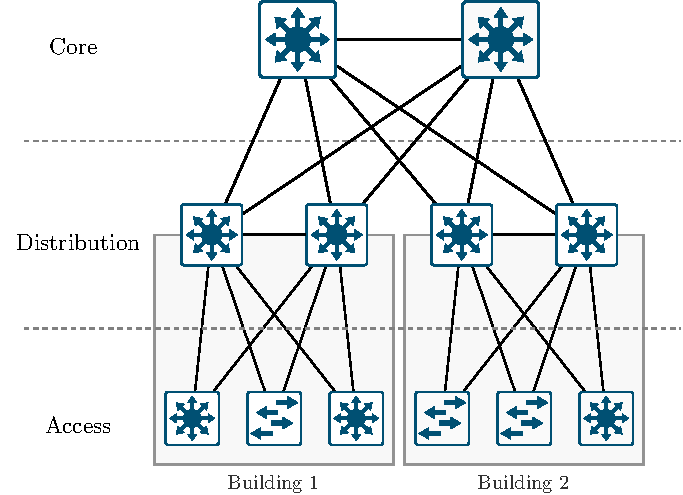
\includegraphics[width=.6\textwidth]{three_layer_model.pdf}
    \end{center}
    \caption{Hierarchical three-layer internetworking model (based on
    \cite{cisco_3_tier})}
    \label{fig:three-layer}
\end{figure}


The architecture of our testbed aligns with the previously design goals,
    achieved through the implementation of the hierarchical three-layer model.

The testbed comprises 205 nodes consisting of 39 routers and 165 end devices.
The network is divided into 4 domains, each potentially representing distinct
    buildings on a university campus.
All 4 domains encompass 7-9 client networks, accommodating 5 end devices each.
The access layer of each domain comprises up to 7 routers (3-digit router IDs
    in \autoref{fig:topology}).
Since this thesis evaluates a transport protocol, we waive the application of
    switches on the access layer, deploying solely  layer 3 devices.
The distribution layer of each domain encompasses 2-3 interconnected routers
    (2-digit router IDs), aggregating the access layers within its respective
    domain and facilitating the connection to the core layer.
The testbed's core consists of 4 routers (1-digit router IDs) interconnecting
    the 4 network domains.
Additionally, the backbone possesses a high connectivity, ensuring both high
    availability and redundancy.
To reduce management and operational overhead, the testbed incorporates fewer
    redundant links from the access to the distribution layer and from the
    distribution to the core layer compared to the recommendations provided by
    Cisco and Huawei \cite{cisco_design_guide,huawei_campus_net}.
This trade-off is considered acceptable, as this thesis does not delve into the
    details of the availability and fault tolerance of the network
    architecture.
Additionally, router and link failures are artificially induced in any case.

The chosen architecture represents a realistic medium-sized network topology.
The application of the hierarchical three-layer model ensures the required
    flexibility of the testbed.
Various placements of senders, receivers, and routers are possible, allowing
    experiments with a receiver distribution ranging from high clustering
    within a single domain to a uniform spread across all four network domains.
Moreover, the availability of alternative routes facilitates the representation
    of dynamic network environments, encompassing scenarios such as deliberate
    routing changes or router and link outages.

\begin{figure}
    \begin{center}
        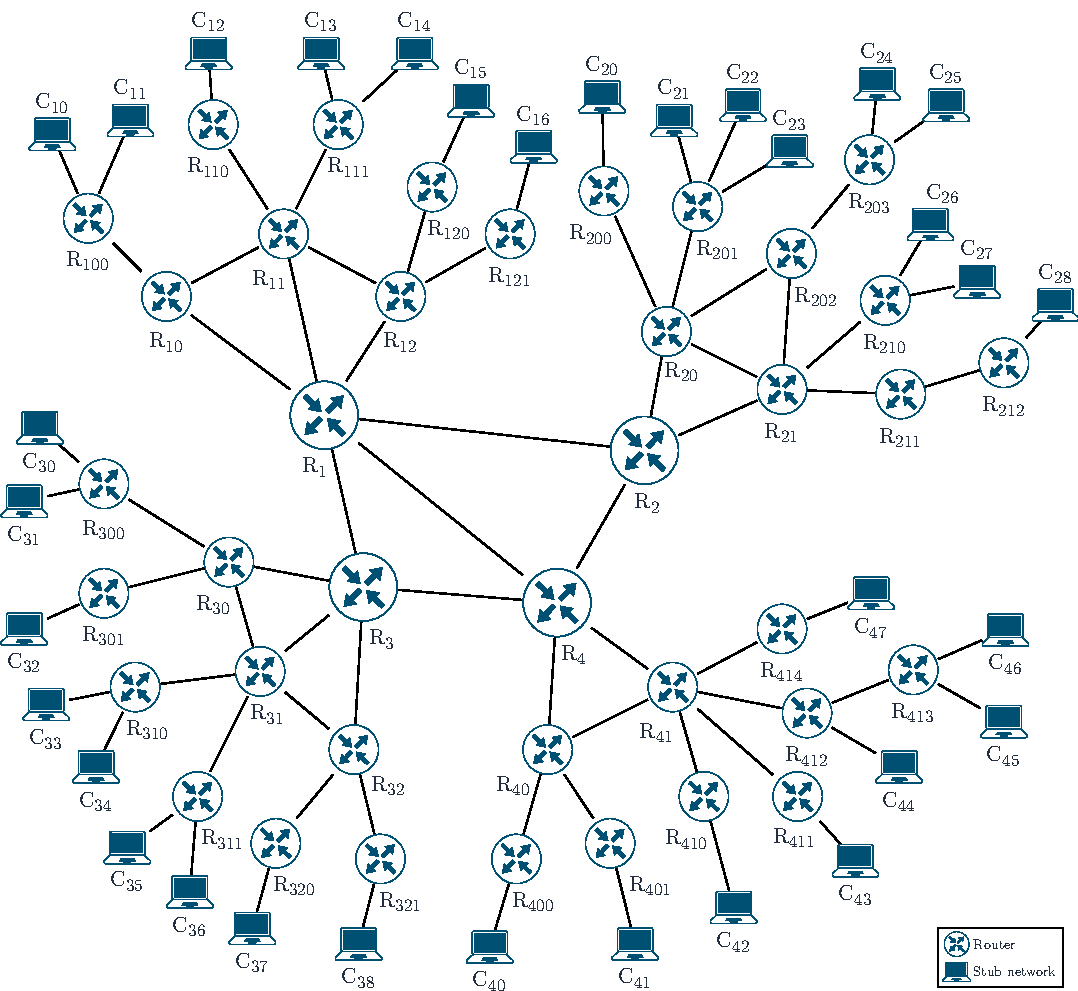
\includegraphics[width=.9\textwidth]{testbed_topology.pdf}
    \end{center}
    \caption{Testbed Topology}
    \label{fig:topology}
\end{figure}

% subsection Topology (end)
% section T (end)


% chapter Design (end)
